\documentclass{standalone}
\usepackage{tikz}
\usetikzlibrary{patterns, positioning}


\begin{document}
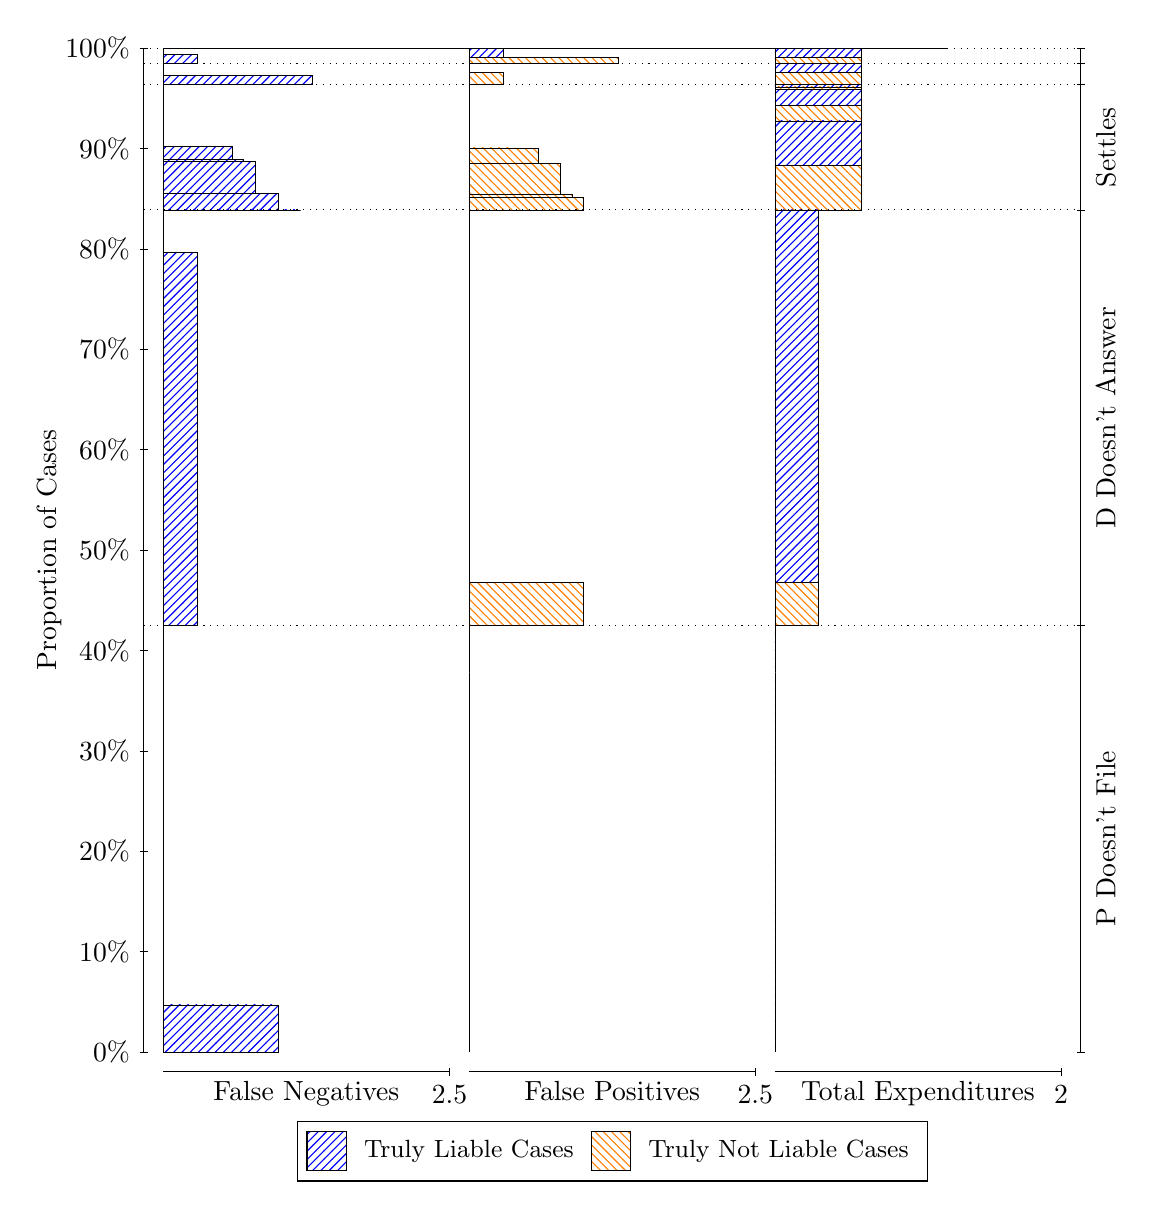
\begin{tikzpicture}
\draw[black, very thin] (1.5,1.75) -- (1.5,14.5);
\node[rotate=90, text=black, anchor=center] at (0.3, 8.125) {Proportion of Cases};
\draw[black, very thin] (1.45,1.75) -- (1.55,1.75);
\node[text=black, anchor=east] at (1.45, 1.75) {0\%};
\draw[black, very thin] (1.45,3.025) -- (1.55,3.025);
\node[text=black, anchor=east] at (1.45, 3.025) {10\%};
\draw[black, very thin] (1.45,4.3) -- (1.55,4.3);
\node[text=black, anchor=east] at (1.45, 4.3) {20\%};
\draw[black, very thin] (1.45,5.575) -- (1.55,5.575);
\node[text=black, anchor=east] at (1.45, 5.575) {30\%};
\draw[black, very thin] (1.45,6.85) -- (1.55,6.85);
\node[text=black, anchor=east] at (1.45, 6.85) {40\%};
\draw[black, very thin] (1.45,8.125) -- (1.55,8.125);
\node[text=black, anchor=east] at (1.45, 8.125) {50\%};
\draw[black, very thin] (1.45,9.4) -- (1.55,9.4);
\node[text=black, anchor=east] at (1.45, 9.4) {60\%};
\draw[black, very thin] (1.45,10.675) -- (1.55,10.675);
\node[text=black, anchor=east] at (1.45, 10.675) {70\%};
\draw[black, very thin] (1.45,11.95) -- (1.55,11.95);
\node[text=black, anchor=east] at (1.45, 11.95) {80\%};
\draw[black, very thin] (1.45,13.225) -- (1.55,13.225);
\node[text=black, anchor=east] at (1.45, 13.225) {90\%};
\draw[black, very thin] (1.45,14.5) -- (1.55,14.5);
\node[text=black, anchor=east] at (1.45, 14.5) {100\%};

\draw[black, very thin] (13.4,1.75) -- (13.4,14.5);
\draw[black, very thin] (13.35,1.75) -- (13.45,1.75);
\node[anchor=west] at (13.35, 1.75) {};
\draw[black, very thin] (13.35,7.1656) -- (13.45,7.1656);
\node[anchor=west] at (13.35, 7.1656) {};
\draw[black, very thin] (13.35,12.444) -- (13.45,12.444);
\node[anchor=west] at (13.35, 12.444) {};
\draw[black, very thin] (13.35,14.039) -- (13.45,14.039);
\node[anchor=west] at (13.35, 14.039) {};
\draw[black, very thin] (13.35,14.307) -- (13.45,14.307);
\node[anchor=west] at (13.35, 14.307) {};
\draw[black, very thin] (13.35,14.497) -- (13.45,14.497);
\node[anchor=west] at (13.35, 14.497) {};
\draw[black, very thin] (13.35,14.498) -- (13.45,14.498);
\node[anchor=west] at (13.35, 14.498) {};
\draw[black, very thin] (13.35,14.5) -- (13.45,14.5);
\node[anchor=west] at (13.35, 14.5) {};

\draw[black, very thin, pattern color=blue, pattern=north east lines] (1.75,1.75) rectangle (3.2033,2.3482);
\draw[black, very thin, pattern color=orange, pattern=north west lines] (1.75,2.3482) rectangle (1.75,7.1656);
\draw[black, very thin, pattern color=blue, pattern=north east lines] (1.75,7.1656) rectangle (2.186,11.9);
\draw[black, very thin, pattern color=orange, pattern=north west lines] (1.75,11.9) rectangle (1.75,12.444);
\draw[black, very thin, pattern color=blue, pattern=north east lines] (1.75,12.444) rectangle (3.494,12.444);
\draw[black, very thin, pattern color=blue, pattern=north east lines] (1.75,12.444) rectangle (3.3487,12.444);
\draw[black, very thin, pattern color=blue, pattern=north east lines] (1.75,12.444) rectangle (3.2033,12.652);
\draw[black, very thin, pattern color=blue, pattern=north east lines] (1.75,12.652) rectangle (3.058,12.653);
\draw[black, very thin, pattern color=blue, pattern=north east lines] (1.75,12.653) rectangle (3.058,12.653);
\draw[black, very thin, pattern color=blue, pattern=north east lines] (1.75,12.653) rectangle (2.9127,13.056);
\draw[black, very thin, pattern color=blue, pattern=north east lines] (1.75,13.056) rectangle (2.7673,13.087);
\draw[black, very thin, pattern color=blue, pattern=north east lines] (1.75,13.087) rectangle (2.622,13.251);
\draw[black, very thin, pattern color=orange, pattern=north west lines] (1.75,13.251) rectangle (1.75,14.039);
\draw[black, very thin, pattern color=blue, pattern=north east lines] (1.75,14.039) rectangle (3.6393,14.157);
\draw[black, very thin, pattern color=orange, pattern=north west lines] (1.75,14.157) rectangle (1.75,14.307);
\draw[black, very thin, pattern color=blue, pattern=north east lines] (1.75,14.307) rectangle (2.186,14.421);
\draw[black, very thin, pattern color=orange, pattern=north west lines] (1.75,14.421) rectangle (1.75,14.497);
\draw[black, very thin, pattern color=blue, pattern=north east lines] (1.75,14.497) rectangle (5.8193,14.497);
\draw[black, very thin, pattern color=orange, pattern=north west lines] (1.75,14.497) rectangle (1.75,14.498);
\draw[black, very thin, pattern color=orange, pattern=north west lines] (1.75,14.498) rectangle (1.75,14.499);
\draw[black, very thin, pattern color=blue, pattern=north east lines] (1.75,14.499) rectangle (1.75,14.5);
\draw[black, very thin, pattern color=orange, pattern=north west lines] (5.6333,1.75) rectangle (5.6333,6.5674);
\draw[black, very thin, pattern color=blue, pattern=north east lines] (5.6333,6.5674) rectangle (5.6333,7.1656);
\draw[black, very thin, pattern color=orange, pattern=north west lines] (5.6333,7.1656) rectangle (7.0867,7.709);
\draw[black, very thin, pattern color=blue, pattern=north east lines] (5.6333,7.709) rectangle (5.6333,12.444);
\draw[black, very thin, pattern color=orange, pattern=north west lines] (5.6333,12.444) rectangle (7.0867,12.608);
\draw[black, very thin, pattern color=orange, pattern=north west lines] (5.6333,12.608) rectangle (6.9413,12.637);
\draw[black, very thin, pattern color=orange, pattern=north west lines] (5.6333,12.637) rectangle (6.796,13.037);
\draw[black, very thin, pattern color=orange, pattern=north west lines] (5.6333,13.037) rectangle (6.6507,13.038);
\draw[black, very thin, pattern color=orange, pattern=north west lines] (5.6333,13.038) rectangle (6.5053,13.23);
\draw[black, very thin, pattern color=orange, pattern=north west lines] (5.6333,13.23) rectangle (6.36,13.23);
\draw[black, very thin, pattern color=orange, pattern=north west lines] (5.6333,13.23) rectangle (6.2147,13.231);
\draw[black, very thin, pattern color=blue, pattern=north east lines] (5.6333,13.231) rectangle (5.6333,14.039);
\draw[black, very thin, pattern color=orange, pattern=north west lines] (5.6333,14.039) rectangle (6.0693,14.189);
\draw[black, very thin, pattern color=blue, pattern=north east lines] (5.6333,14.189) rectangle (5.6333,14.307);
\draw[black, very thin, pattern color=orange, pattern=north west lines] (5.6333,14.307) rectangle (7.5227,14.383);
\draw[black, very thin, pattern color=blue, pattern=north east lines] (5.6333,14.383) rectangle (6.0693,14.497);
\draw[black, very thin, pattern color=orange, pattern=north west lines] (5.6333,14.497) rectangle (5.6333,14.497);
\draw[black, very thin, pattern color=blue, pattern=north east lines] (5.6333,14.497) rectangle (5.6333,14.498);
\draw[black, very thin, pattern color=orange, pattern=north west lines] (5.6333,14.498) rectangle (9.7027,14.499);
\draw[black, very thin, pattern color=blue, pattern=north east lines] (5.6333,14.499) rectangle (8.2493,14.5);
\draw[black, very thin, pattern color=orange, pattern=north west lines] (9.5167,1.75) rectangle (9.5167,6.5674);
\draw[black, very thin, pattern color=blue, pattern=north east lines] (9.5167,6.5674) rectangle (9.5167,7.1656);
\draw[black, very thin, pattern color=orange, pattern=north west lines] (9.5167,7.1656) rectangle (10.062,7.709);
\draw[black, very thin, pattern color=blue, pattern=north east lines] (9.5167,7.709) rectangle (10.062,12.444);
\draw[black, very thin, pattern color=orange, pattern=north west lines] (9.5167,12.444) rectangle (10.607,13.009);
\draw[black, very thin, pattern color=blue, pattern=north east lines] (9.5167,13.009) rectangle (10.607,13.576);
\draw[black, very thin, pattern color=orange, pattern=north west lines] (9.5167,13.576) rectangle (10.607,13.769);
\draw[black, very thin, pattern color=blue, pattern=north east lines] (9.5167,13.769) rectangle (10.607,13.978);
\draw[black, very thin, pattern color=orange, pattern=north west lines] (9.5167,13.978) rectangle (10.607,14.007);
\draw[black, very thin, pattern color=blue, pattern=north east lines] (9.5167,14.007) rectangle (10.607,14.039);
\draw[black, very thin, pattern color=orange, pattern=north west lines] (9.5167,14.039) rectangle (10.607,14.189);
\draw[black, very thin, pattern color=blue, pattern=north east lines] (9.5167,14.189) rectangle (10.607,14.307);
\draw[black, very thin, pattern color=orange, pattern=north west lines] (9.5167,14.307) rectangle (10.607,14.383);
\draw[black, very thin, pattern color=blue, pattern=north east lines] (9.5167,14.383) rectangle (10.607,14.497);
\draw[black, very thin, pattern color=orange, pattern=north west lines] (9.5167,14.497) rectangle (11.697,14.497);
\draw[black, very thin, pattern color=blue, pattern=north east lines] (9.5167,14.497) rectangle (11.697,14.498);
\draw[black, very thin, pattern color=orange, pattern=north west lines] (9.5167,14.498) rectangle (11.697,14.499);
\draw[black, very thin, pattern color=blue, pattern=north east lines] (9.5167,14.499) rectangle (11.697,14.5);
\draw[black, dotted] (1.5,7.1656) -- (13.4,7.1656);
\draw[black, dotted] (1.5,12.444) -- (13.4,12.444);
\draw[black, dotted] (1.5,14.039) -- (13.4,14.039);
\draw[black, dotted] (1.5,14.307) -- (13.4,14.307);
\draw[black, dotted] (1.5,14.497) -- (13.4,14.497);
\draw[black, dotted] (1.5,14.498) -- (13.4,14.498);
\draw[black, very thin] (1.75,1.5) -- (5.3833,1.5);
\node[text=black, anchor=north] at (3.5667, 1.5) {False Negatives};
\draw[black, very thin] (5.3833,1.45) -- (5.3833,1.55);
\node[text=black, anchor=north] at (5.3833, 1.45) {2.5};

\draw[black, very thin] (5.6333,1.5) -- (9.2667,1.5);
\node[text=black, anchor=north] at (7.45, 1.5) {False Positives};
\draw[black, very thin] (9.2667,1.45) -- (9.2667,1.55);
\node[text=black, anchor=north] at (9.2667, 1.45) {2.5};

\draw[black, very thin] (9.5167,1.5) -- (13.15,1.5);
\node[text=black, anchor=north] at (11.333, 1.5) {Total Expenditures};
\draw[black, very thin] (13.15,1.45) -- (13.15,1.55);
\node[text=black, anchor=north] at (13.15, 1.45) {2};

\node[text=black, centered, rotate=90] at (13.72, 4.4578) {P Doesn't File};
\node[text=black, centered, rotate=90] at (13.72, 9.8046) {D Doesn't Answer};
\node[text=black, centered, rotate=90] at (13.72, 13.241) {Settles};





\draw (7.449999999999999,1.5) node[draw=none] (baseCoordinate) {};
\begin{scope}[align=center]
        \matrix[scale=0.5, draw=black, below=0.5cm of baseCoordinate, nodes={draw}, column sep=0.1cm]{
            \node[rectangle, draw, minimum width=0.5cm, minimum height=0.5cm, pattern color=blue, pattern=north east lines] {}; &
            \node[draw=none, font=\small, text=black] (B) {Truly Liable Cases}; &
            \node[rectangle, draw, minimum width=0.5cm, minimum height=0.5cm, pattern color=orange, pattern=north west lines] {}; &
            \node[draw=none, font=\small, text=black] (B) {Truly Not Liable Cases}; \\
            };
\end{scope}

\end{tikzpicture}
\end{document}